\section{Comparison}
\label{sec:comparison}

% original paper
The authors of \cite{SNN}  present an unsupervised approach to train a \ac{SNN} model.
However, there are other approaches to train \acp{SNN}, as well as opinions with regard to the biological plausibility of the methods used.
In the following, the \ac{SNN} model from \cite{SNN} is compared to other \ac{SNN} models.


% STDP-like paper
The presented \ac{SNN} model determines its output by 
choosing the class of the first neuron pool to reach the decision threshold with its accumulated sensory evidence \cite{STDP_like}.
The authors claim that the original method of using a majority vote of single threshold-based neuron activity is less biologically plausible.

Not only the \cite{STDP_like} model but also the \cite{SNN} model use inhibition.
\todo{zitierung als satzbaustein. Wie sonst?}

The authors of \cite{STDP_like} point out that the classifier neurons will not recognize atypical digits (i.e. their stimulus).
Therefore, the ability to generalize on new datasets depends on the inputs' similarity to the learned patterns.


% DIET-SNN paper

% Captial L to avoid strange behaviour since the figure is close to the page break
%\begin{wrapfigure}{L}{0.25\textwidth}
%    \centering
%    \vspace{-20pt}
%    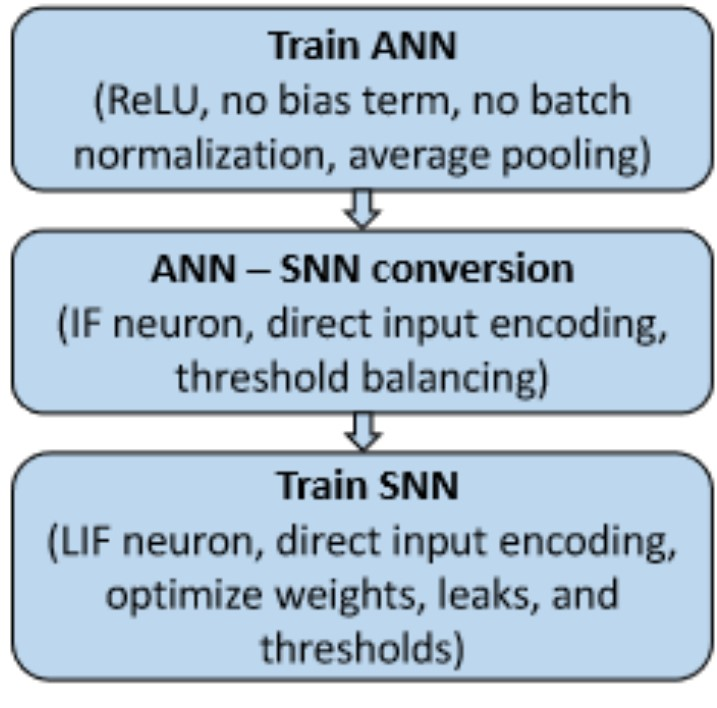
\includegraphics[width=0.25\textwidth]{pictures/DIET_SNN_pipeline.jpg}
%    \caption{\acs{DIET}-\ac{SNN} training pipeline from \cite{DIET_SNN}.}
%    \label{fig:training_pipeline_DIET_SNN}
%\end{wrapfigure}

%\todo{ich weiß zwar nicht wie, aber die figure sollte auf der gleichen höhe wie der text beginnen}
%The \ac{DIET}-\ac{SNN} model from \cite{DIET_SNN} is an entirely different approach to those discussed before.
%This alternative approach uses supervised learning.
%\todo{warum kommt hier ein neues model hinzu? hatten Sie sorge, dass sie nicht
%  auf die benötigte seitenzahl kommen? dieser sprung zu einem weiteren model
%  ohne vorherige erwähnung bringt einen ganz schön in verwirrung}
%\todo{da die seitenzahl sowieso schon etwas über dem limit ist, wäre hier ein
%  guter ansatz um die arbeit etwas zu kürzen}
\todo{am anfang 3/4 features/eigenschaften erwähnen/erklären, die verglichen
  werden sollen und dann kurz ein weiteres model nehmen oder besser noch nur mit
  klassische nn und vergleichen}
%As depicted in \autoref{fig:training_pipeline_DIET_SNN}, an \ac{ANN} is trained and thereafter converted into a \ac{SNN}.
%The \ac{ANN}-\ac{SNN}-conversion is outlined in \cite{DIET_SNN} and \cite{ANN_SNN_conversion}.
%The initialized parameters speed up the subsequent training of the converted \ac{SNN} with spike-based error-backpropagation.

%Instead of using a Poisson generator (i.e. rate-coding: converting analog values to spike-train), the image pixels are directly applied as input.
%The \ac{DIET}-\ac{SNN} model's first layer is trained to encode the input as spikes.
%The pixel intensities of an image are directly applied to the first convolutional layer's \ac{LIF} neurons.
%The neurons accumulate the weighted pixel and generate output spikes.
%This encoding is learned beforehand using gradient descent.

%\todo{irgendwie kriegt man das centering hier bestimmt hin}
%\begin{equation}
%    \centering
%    \label{eq:DIET-SNN-membrane-potential}
%    u_i^t = \lambda_i u_i^{t-1} + \sum_{j}^{}w_{ij}o_j^t-v_{i}o_i^{t-1}
%\end{equation}
%
%The membrane potential $u_i^t$ of a postsynaptic neuron $i$ at timestep $t$ 
%is calculated using \autoref{eq:DIET-SNN-membrane-potential} from \cite{DIET_SNN}. 
%$\lambda_i \in [0,1]$ is the leak factor of the membrane potential, 
%\todo{einen satz mit einem mathematischen symbol anfangen ist nicht so gut}
%$w_{ij}$ the weight of the synapse between neuron $i$ and $j$, 
%$o_j^t$ the output spike of neuron $j$ at timestep $t$ and 
%$v_i$ the threshold of neuron $i$.
%The first term calculates the leakage of the neuron,
%the second term the accumulated input of the presynaptic neurons and
%the third term enables a soft reset (reducing by threshold $v_i$ instead of reset to zero) of the membrane potential after a spike was generated.
%The neurons of the output layer accumulate their inputs without any leakage.
%The output is not a spike, but a softmax function of the membrane potential.

% multi_scale_STDP paper
The model presented both in \cite{multi_scale_STDP} and \cite{STDP_vis_feat} is different than \cite{SNN}.
It is designed to execute object recognition tasks in a biologically plausible manner.

The first difference is the architecture \cite{multi_scale_STDP,STDP_vis_feat}.
%usage of a five-layer hierarchical network structure, consisting of alternating so-called simple cells $S_1, S_2$ and complex cells $C_1, C_2$.
%The simple cells employ intensity-to-latency conversion, i.e. the stronger a cell is stimulated the earlier it will fire \cite{STDP_vis_feat}.
%In a group of four simple cells, the cell with the earliest firing time inhibits the other cells and thus, creating winner-take-all inhibition \cite{multi_scale_STDP}.
%The spike omitted by the winner cell is then propagated asynchronously.
%It serves as input for the complex cells.
%Since there are fewer complex cells than simple ones, the complex cells propagate only the maximum, i.e. the earliest spike \cite{STDP_vis_feat}, of the input spikes.

%The second difference is the use of a classifier in the fifth layer to carry out the classification task 
The second difference is the use of a classifier to carry out the classification task 
instead of deciding on the class whose neurons have the highest average firing rate, 
as suggested by the authors of \cite{SNN}.

Moreover, the model has a multi-scale form \cite{multi_scale_STDP}.
In other words: 
The original image is scaled to different processing scales (100\%, 71\%, 50\%, 30\% and 25\%) and parallelly processed until 
all processing scales are combined in one of the layers.
%the fourth layer.

However, there are also similarities to the \cite{SNN} model:
%The $C_1$ to $S_2$ synaptic connections are trained using \ac{STDP} \cite{multi_scale_STDP,STDP_vis_feat}.
The synaptic connections are trained using \ac{STDP} \cite{multi_scale_STDP,STDP_vis_feat}.
Yet, the time difference between the presynaptic and postsynaptic spike is only used to determine the sign of the modification of the synaptic weight 
but is not relevant for the amount of weight change \cite{STDP_vis_feat}.
As mentioned before, both the \cite{multi_scale_STDP} and the \cite{SNN} model use inhibition and thus, 
create competition and consequently ensure all neurons learn a distinct pattern to cover the whole variability of inputs \cite{STDP_vis_feat}.
%
The \cite{multi_scale_STDP} model is trained and evaluated on the ETH-80 and 3D-Object datasets \cite{multi_scale_STDP}, which contain objects with large deviations.
The data is converted to grayscale values.
A \ac{RDM} is used to determine whether the quality of the model is good enough to provide a representation of objects which have a high inter-category dissimilarity and a low intra-category dissimilarity.
The result of the \ac{RDM} in \autoref{fig:RDM_SNN} suggests that the model is able to distinguish between feature values of different categories.
The authors include a \ac{RDM} of a non-\ac{SNN} model performing considerably worse.
%
\begin{figure}[htbp]
    \center
    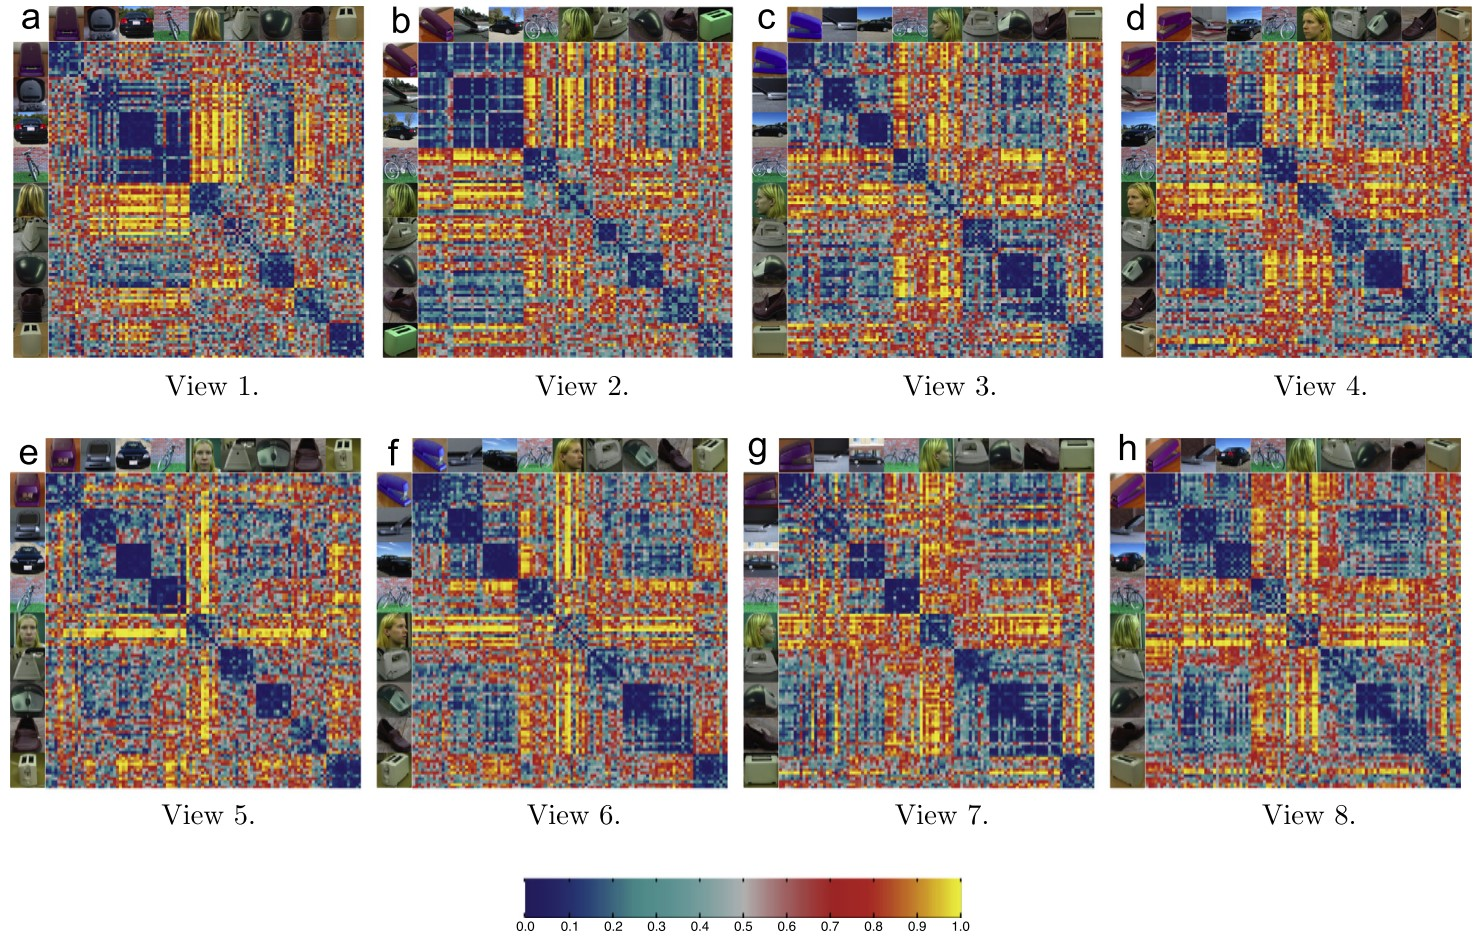
\includegraphics[width=0.9\textwidth]{pictures/inter_intra_category_dissimilarity.jpg}
    \caption{\acp{RDM} of object representations of different image stimuli for different views from \cite{multi_scale_STDP}.
    A sample image for each category is placed next to the rows and columns.
    Intra-class dissimilarity is low, and inter-class dissimilarity is high.}
    \label{fig:RDM_SNN}
\end{figure}
%
The model becomes selective to the prominently present patterns in the input and generates fast responses \cite{STDP_vis_feat}.
The multi-scale \ac{SNN} is well suited for object recognition tasks consisting of few classes and many viewpoints \cite{multi_scale_STDP}.
The authors admit that processing time for many classes would greatly increase.

% triplet-based STDP paper
The authors of \cite{STDP_triplet} claim that classical pair based \ac{STDP} models 
are not able to explain synaptic changes caused by triplets or quadruplets of spikes.